%=====================================================
\begin{frame}{3.2.3. Частотность обращения педагогов к администрации по вопросам преподавания и воспитания (группы по квалификационной категории) }

\tiny

На диаграммах представлен результат по вопросам Б15, Б16, Б17 с разбивкой по квалификационной категории:
\bigskip

\centering 

\begin{tabular}{|l|c|c|c|c|c|} \hline
  & Не проходил &  Аттестован & 2-я &  1-я  & Высшая \\ 
 &  аттестацию   &  на соотв. & категория &  категория  & категория \\ \hline
Ответили  & & & & & \\
утвердительно  & \valCBCyesNumA  & \valCBCyesNumB  & \valCBCyesNumC & 
\valCBCyesNumD  & \valCBCyesNumE  \\ 
(Раз в месяц или чаще) & & & & & \\ \hline
Ответили   & & & & & \\
отрицательно & \valCBCnoNumA & \valCBCnoNumB  &  \valCBCnoNumC  & 
\valCBCnoNumD & \valCBCnoNumE \\ 
(Раз в полугодие или реже) & & & & & \\ \hline
\end{tabular}

\bigskip

\begin{tabular}{ccccc}
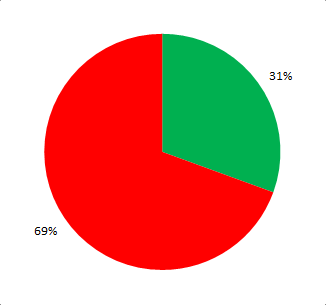
\includegraphics[width=2cm, height=2cm]{diag.png} & 
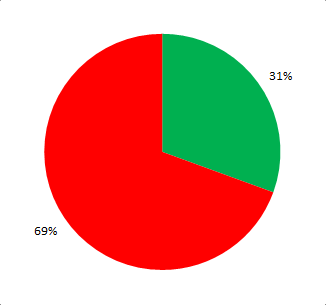
\includegraphics[width=2cm, height=2cm]{diag.png} & 
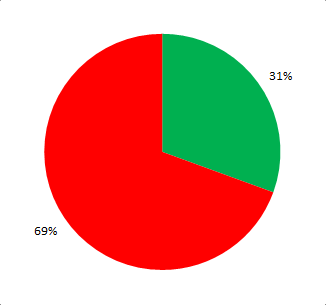
\includegraphics[width=2cm, height=2cm]{diag.png} & 
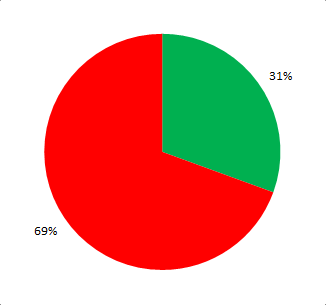
\includegraphics[width=2cm, height=2cm]{diag.png} & 
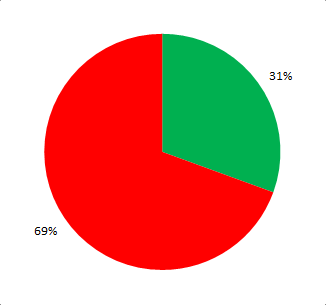
\includegraphics[width=2cm, height=2cm]{diag.png} \\
 Не проходили &  Аттестованы & 2-я &  1-я  & Высшая \\ 
  аттестацию   &  на соотв. & категория &  категория  & категория \\ 
\end{tabular}

\end{frame}


